\documentclass[10pt,a4paper]{article}

\usepackage{amsmath}
\usepackage{amsfonts}
\usepackage{amssymb}
\usepackage{booktabs}
\usepackage[margin=2.5cm]{geometry}
\usepackage{graphicx}

\author{B00902031 Kevin Tsai, B00902107 Suhorng You}
\title{CN HW2 report}

\begin{document}

\maketitle

\section{Introduction}
    In this homework, we have implemented a modification of Go-Back-N protocol with partially realized connection management. The sender transmits $8$ packets without waiting for acknowledgements of each packet. To simplify the design, in each connection, data to be sent is given to the sender as a stream, and \texttt{rdt\_send} is automatically invoked by the sender when the window is empty to refill the window by data from the stream. Similar changes is made to the receiver. When called, the receiver blocks and wait until a transmission came, and it automatically allocates memory to store data, returns when all data has arrived.

    We also add connection termination control to both sender and receiver to handle when to end a transmission. The connection termination phase is drawn from that of the TCP's, except that we use a three-way handshake since the connection is unidirectional.

    ``make'' compiles two binary files: ``sender'' and ``receiver.'' Start receiver at the target computer, and then execute sender to send the file. The file sent will be saved at the working directory of sender, which is normally the directory sender is in. Filename and file permissions are preserved during the transmission. If there already exists a file with the same name, the transmission will be terminated. Sender closes after the transmission.

    Command line arguments is as follows:
\begin{verbatim}
$ make											build targets
$ make clean									clean targets and object files
$ ./sender TARGET_HOSTNAME TARGET_IP FILENAME	send file
$ ./receiver LISTEN_PORT						receive files, waiting at port LISTEN_PORT
\end{verbatim}

    The receiver continues to receive files after previous transfer has ended until a \texttt{\^{}C} is hit. Transferring multiple files simultaneously is not support, however.
\section{Unreliable Data Transfer Layer}
    This layer simply uses UDP to transfer data. This layer provides functions to open UDP sockets, to send packages to and receives packages from the socket, and to close the socket. This layer also provides an additional function that clears the socket buffer in case that there are any redundant packages left in the socket.
    % POSSIBLY TODO: WHAT HAVE WE DONE TO THE UDP SOCKET? FUNCTIONALITY OF udt.cpp?

\section{Reliable Data Transfer Layer}
\subsection{Packet Format}
    The size of packets varies from $9$ bytes to $256$ bytes. The first byte of the packet specifies the size of the following data, that is, $8$ bytes plus the length of the content. It is followed by a $4$-byte unsigned integer sequence number, and a $4$-byte unsigned int CRC-32 checksum. The rest are the actual data that we want to transfer, whose length could be from $1$ byte to $247$ bytes.

\begin{center}
    \begin{tabular}{lcc}
        Entry Name & Size (bytes) & Interpretation \\%& Type & Meaning\\
            \hline
        packet size & $1$ &  size of the packet (exclusive of this entry)\\ 
        sequence number & $4$ & sequence number of the packet\\
        checksum & $4$ & the CRC-32 checksum of the whole package, with this entry treated as zero\\
        data & $1$-$247$ & the data being transferred\\
    \end{tabular}
\end{center}

    
\subsection{Receiver and Sender FSM}
    \begin{center}
        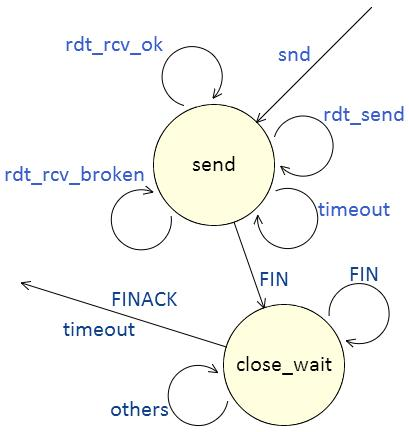
\includegraphics[scale=0.7]{fsmsnd.jpg}
        \; \; \;
        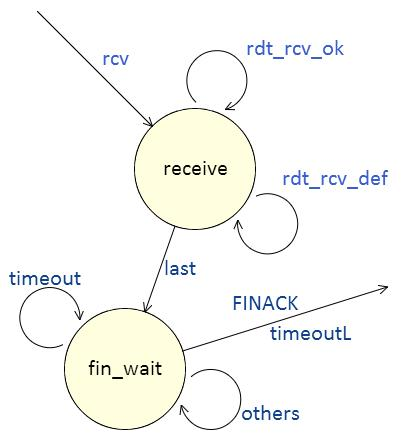
\includegraphics[scale=0.7]{fsmrcv.jpg}
    \end{center}
    \subsubsection{Sender}
    \begin{enumerate}
    	\item \texttt{snd}:
        \item \texttt{rdt\_send}:
        \item \texttt{rdt\_rcv\_ok}:
        \item \texttt{rdt\_rcv\_broken}:
        \item \texttt{timeout}:
        \item \texttt{send::FIN}:
        \item \texttt{others}:
        \item \texttt{close\_wait::FIN}:
        \item \texttt{FINACK}, \texttt{close\_wait::timeout}:
    \end{enumerate}
    \subsubsection{Receiver}
    \begin{enumerate}
        \item \texttt{rcv}:
        \item \texttt{rdt\_rcv\_ok}:
        \item \texttt{rdt\_rcv\_def}:
        \item \texttt{last}:
        \item \texttt{timeout}:
        \item \texttt{others}:
        \item \texttt{FINACK}, \texttt{timeoutL}:
    \end{enumerate}
\subsection{Protocol}
\section{Loss and error solving}
    \subsection{Packet loss solving}
        Nice question, horrible solution.
    \subsection{Packet error solving}
        There is a checksum in every packet sent. When received, the program checks if the checksum in the package is correct. Corrupted packets are ignored. The use of CRC-32 which is based on cyclic error-checking codes guarantees low error rate.

\section{Application Layer}
\section{Extra work}
    %% maybe FIN is extra work?
\section{Snapshots}
\end{document}